\input{"C:/Users/spileggi/Google Drive/STAT 330/Lectures/SlideStyle.tex"}



\title[Lecture 13]{PROC ANOVA, PROC REG, and PROC GLM}
\author[Pileggi]{Shannon Pileggi}

\institute[STAT 330]{STAT 330}

\date{}


\begin{document}

\begin{frame}
\titlepage
\end{frame}

\begin{frame}
\frametitle{OUTLINE\qquad\qquad\qquad} \tableofcontents[hideallsubsections]
\end{frame}

%===========================================================================================================================
\section[Overview]{Overview}
%===========================================================================================================================
\subsection{}

\begin{frame}
\frametitle{Methods overview}
ANOVA (analysis of variance)
\begin{itemize}
    \item
    Dependent variable = quantitative
    \item[] independent variable = categorical (more than 2 levels)
    \item
    interested in comparing $>$2 groups
    \item[]
    $H_0: \mu_1=\mu_2=\mu_3=\ldots \mu_g$ for $g$ groups
    \item[]
    $H_a$: at least one mean is different than the others
    \item[]
\end{itemize}

Linear Regression
\begin{itemize}
    \item
    Dependent variable = quantitative
    \item[] independent variable(s) = quantitative or categorical
    \item
    interested in examining the relationship between $x$ and $y$
    \item[]
    $H_0$: $\beta_1=0$ vs  $H_a$: $\beta_1 \neq 0$
\end{itemize}
\end{frame}


\begin{frame}
\ft{PROCs Overview}
All can be used to model a \emph{quantitative} dependent variable.
\vskip5pt
\bmp{0.3\textwidth}
\underline{\ttt{PROC REG}}
\bi
\item simple linear regression
\item polynomial regression
\item regression with multiple predictors
\item[]
\item[]
\item[]
\item[]
\item[]
\ei
\emp
\bmp{0.3\textwidth}
\underline{\ttt{PROC ANOVA}}
\bi
\item analysis of variance (for balanced data)
\item multivariate analysis of variance (MANOVA)
\item  repeated measures analysis of variance
\item[]
\item[]
\ei
\emp
\bmp{0.45\textwidth}
\underline{\ttt{PROC GLM}}
\bi
\item  simple regression
\item  multiple regression
\item  analysis of variance
\item  analysis of covariance
\item  response-surface models
\item  weighted regression
\item  polynomial regression
\item  partial correlation
\item  multivariate analysis of variance
\item  repeated measures analysis of variance
\ei
\emp
\end{frame}


\begin{frame}
\ft{Overview, continued}
\bi
\item \ttt{PROC GLM} can do the same type of analyses as \ttt{PROC REG} and \ttt{PROC ANOVA}
\item \ttt{PROC REG} and \ttt{PROC ANOVA} allow you to do more detailed analysis related specifically to regression and \ttt{ANOVA}, respectively
\item all procedures have their quirks...
\ei
\end{frame}

\begin{frame}
\ft{Some quirks}
\resizebox{1.0\textwidth}{!}{
\begin{tabular}{|p{3.5cm} |p{3cm} |p{3cm} |p{3cm}|}
\hline
Feature & \ttt{PROC REG} & \ttt{PROC ANOVA} & \ttt{PROC GLM}\\
\hline
\hline
Dependent var & quantitative & quantitative & quantitative \\
\hline
Quantitative independent var &  \gc & \rx & \gc \\
\hline
Categorical independent var & must be coded as indicator variables in the data set (no \ttt{CLASS} statment) & use \ttt{CLASS} statement & use \ttt{CLASS} statement\\
\hline
Higher order terms (e.g., squares, interactions) & must be coded in the data set & can be written in \ttt{MODEL} statement & can be written in \ttt{MODEL} statement \\
\hline
%\ttt{CLASS} statement & \rx & \gc & \gc \\
%\hline
Multiple \ttt{MODEL} statements & \gc & \rx & \rx \\
\hline
Parameter estimates & automatic & N/A & may need to use \ttt{SOLUTION} option if have categorical ind var\\
\hline
\end{tabular}}
\end{frame}

\begin{frame}
\ft{The Data}
Collected from Kelly Blue Book for 2005 used GM cars
\vskip5pt
\begin{tabular}{r|l}
\ttt{Price} & suggested retail price  \\
\ttt{Mileage} & number of miles the car has been driven  \\
\ttt{Make} & manufacturer of the car   \\
\ttt{Model} & specific models for each car manufacturer  \\
\ttt{Trim} & specific type of car model   \\
\ttt{Type} & body type  \\
\ttt{Cylinder} &  number of cylinders in the engine  \\
\ttt{Liter} & a more specific measure of engine size  \\
\ttt{Doors} &  number of doors  \\
\ttt{Cruise} & whether the car has cruise control (Y/N)  \\
\ttt{Sound} & indicator for upgraded speakers (1 = upgraded)  \\
\ttt{Leather} &  indicator for leather seats (1 = leather)  \\
\end{tabular}
\end{frame}


\begin{frame}[fragile]
\ft{Get started}
\bmp{1.0\textwidth}
\footnotesize
\begin{code}{.0}
LIBNAME flash "&path";

PROC CONTENTS DATA = flash.cars VARNUM ;
RUN;

PROC MEANS DATA = flash.cars ;
   VAR price mileage liter ;
RUN ;

PROC FREQ DATA = flash.cars ;
   TABLES make type cylinder doors cruise sound leather ;
RUN ;
\end{code}
\emp
\end{frame}

\begin{frame}
\frametitle{Review}
\oyo Match the appropriate statistical method for each research question.
\vskip10pt
\bmp{0.35\textwidth}
\be
\item one-sample t-test
\item two sample t-test
\item paired t-test
\item correlation
\item simple linear regression
\item multipe linear regression
\item ANOVA
\ee
\emp
\bmp{0.10\textwidth} \hspace{0.05in} \emp
\bmp{0.55\textwidth}
\begin{enumerate}[]
\item[\underline{\hspace{0.25in}}] Does the population average of price differ by number of doors (2,4) the car comes with?
\item[\underline{\hspace{0.25in}}] Does the population average of price differ by number of cylinders (4,6,8) the car has?
\item[\underline{\hspace{0.25in}}] Is there a relationship between price and mileage?
\item[\underline{\hspace{0.25in}}] Is there a relationship between price and mileage after adjusting for number of doors?
\end{enumerate}
\emp
\end{frame}
%===========================================================================================================================
\section[ANOVA]{ANOVA}
%===========================================================================================================================
\subsection{}
\begin{frame}
\tableofcontents[currentsection, hideallsubsections]
\end{frame}


\begin{frame}
\ft{Review}
\begin{clicker}{Which figure would you produce to examine the relationship between price and number of cylinders (4,6,8)?}
\begin{enumerate}
\item histogram
\item single boxplot
\item side by side boxplot
\item scatter plot
\end{enumerate}
\end{clicker}
\end{frame}




%\begin{frame}
%\frametitle{Conclusion}
%$H_0: \mu_1=\mu_2=\mu_3=\ldots \mu_g$ vs \\
%$H_a$: at least one mean different than the others
%\vskip15pt
%\begin{columns}
%\column{0.5\textwidth}
%\underline{If $p$-value $>\alpha$}
%\begin{itemize}
%    \item
%    fail to reject $H_0$
%    \item
%    there is not sufficient evidence to suggest that population means differ significantly
%     \item[]
%    \item[]
%\end{itemize}
%\column{0.5\textwidth}
%\underline{If $p$-value $\leq\alpha$}
%\begin{itemize}
%    \item
%    reject $H_0$
%    \item
%    there is evidence that at least one population mean differs from the others
%    \item
%    need a post-hoc test to determine which population means differ
%\end{itemize}
%\end{columns}
%\end{frame}
%
%
%
%\begin{frame}
%\frametitle{Multiple testing techniques}
%\begin{itemize}
%    \item
%    When you reject $H_0: \mu_1=\mu_2=\mu_3$ in one-way ANOVA, it is of interest to determine exactly which means differ and to what extent they differ
%    \item
%    This results in \emph{pairwise comparisons}.  If you have 3 groups, there are 3 pairwise comparisons (1-2,1-3,2-3)
%    \item
%    The goal of multiple testing/confidence interval techniques is to \textbf{control} the overall Type I error rate in a \emph{set} of tests or the overall confidence level in a \emph{set} of confidence intervals
%    \item
%    There are many techniques available, including Fisher, Bonferroni, Tukey, scheffe, etc.
%\end{itemize}
%\end{frame}


\begin{frame}[fragile]
\frametitle{Syntax}
\bmp{1.0\textwidth}
\footnotesize
\begin{code}{.0}
PROC ANOVA DATA = \emph{mydata} ;
    CLASS \emph{catvar};
    MODEL \emph{quantvar} = \emph{catvar} ;
    MEANS \emph{catvar}  /  \emph{options} ;
QUIT ;
\end{code}
\emp
\vskip10pt
\bi
\item \ttt{CLASS} - specify categorical independent variable (treatment)
\item \ttt{MODEL} - specify relationship
\item \ttt{MEANS} - estimates means for all levels of \ttt{CLASS} variable
\ei
\end{frame}

\begin{frame}[fragile]
\frametitle{PROC ANOVA Example}
\bmp{0.55\textwidth}
\footnotesize
\begin{code}{.0}
PROC ANOVA DATA = flash.cars ;
   CLASS cylinder ;
   MODEL price = cylinder ;
   MEANS cylinder ;
QUIT ;
\end{code}
\vspace{2ex}
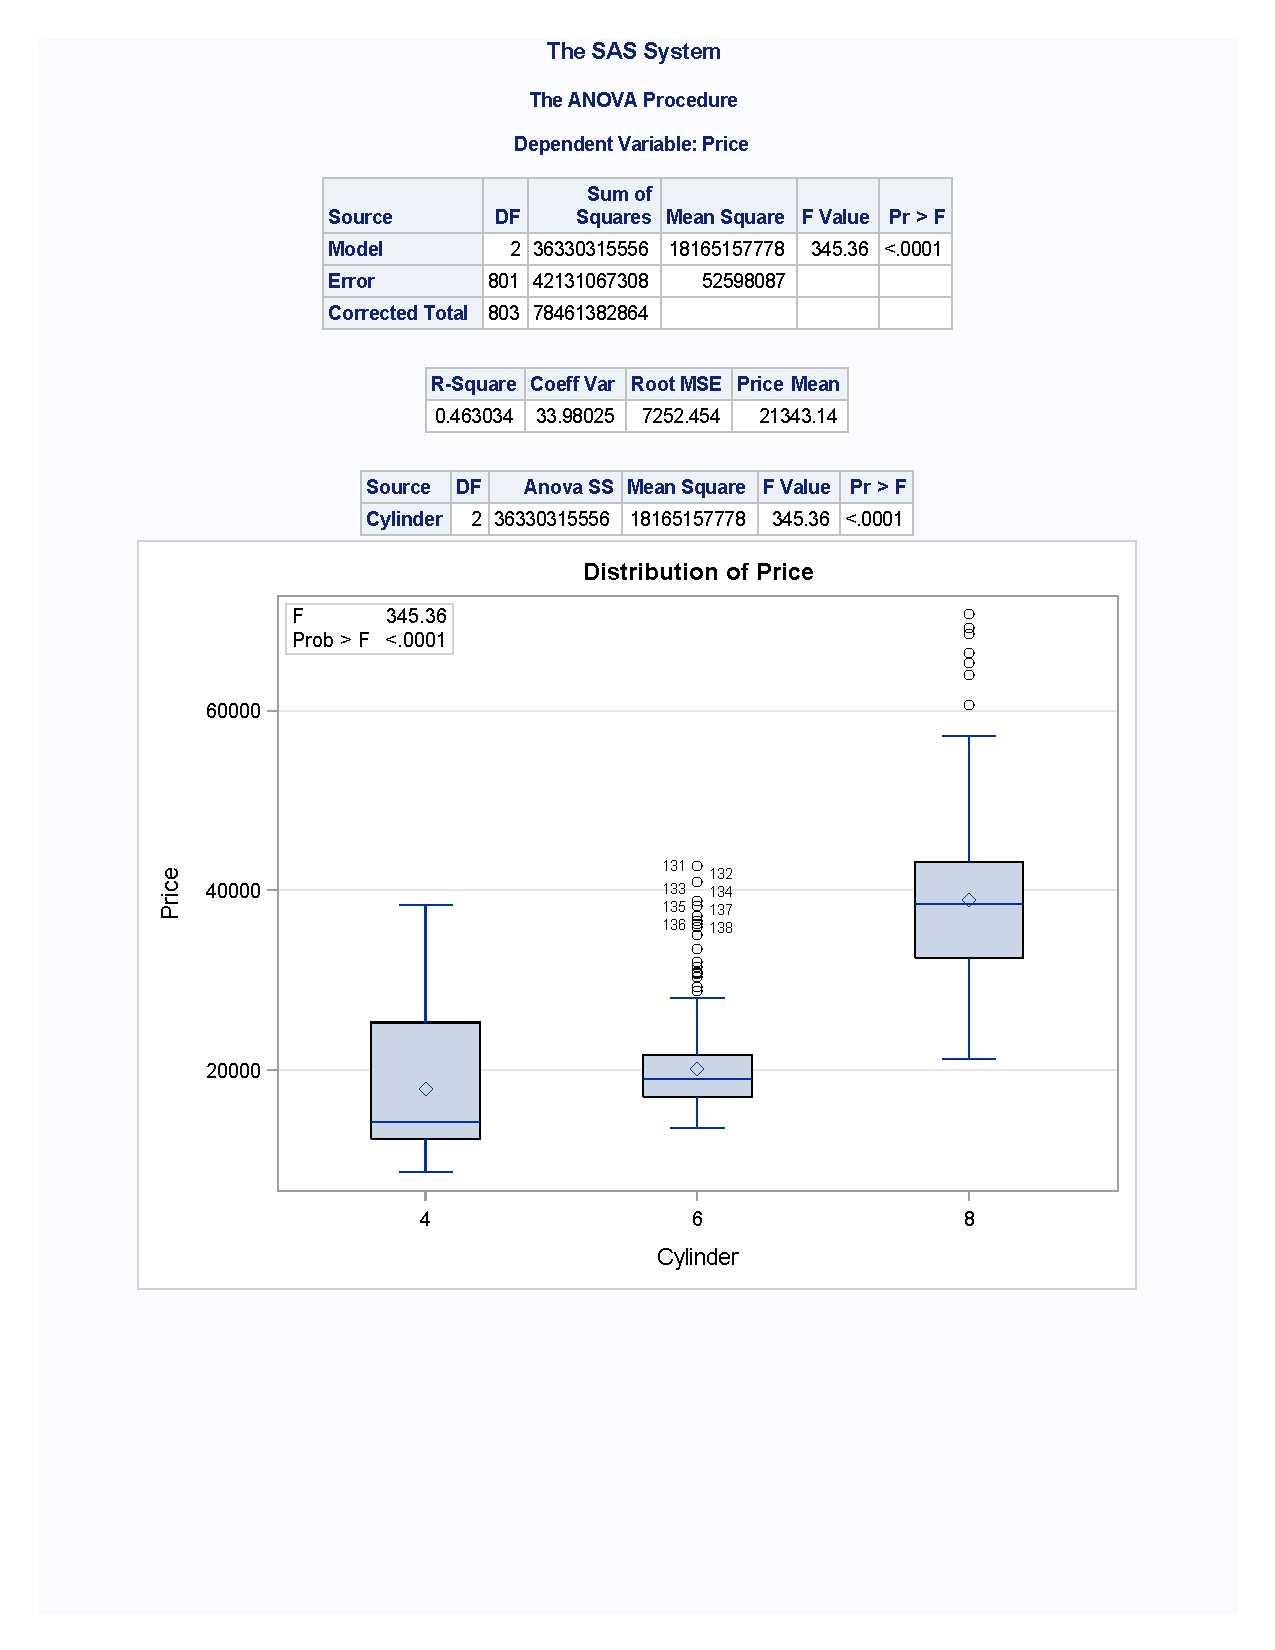
\includegraphics[trim=4cm 18.7cm 4cm 2cm,clip,width=1.0\textwidth]{L13_anova2.pdf}
\emp
\bmp{0.05\textwidth} \hspace{1in} \emp
\bmp{0.45\textwidth}
\oyo What is the next step in this analysis?\\
\vskip49pt
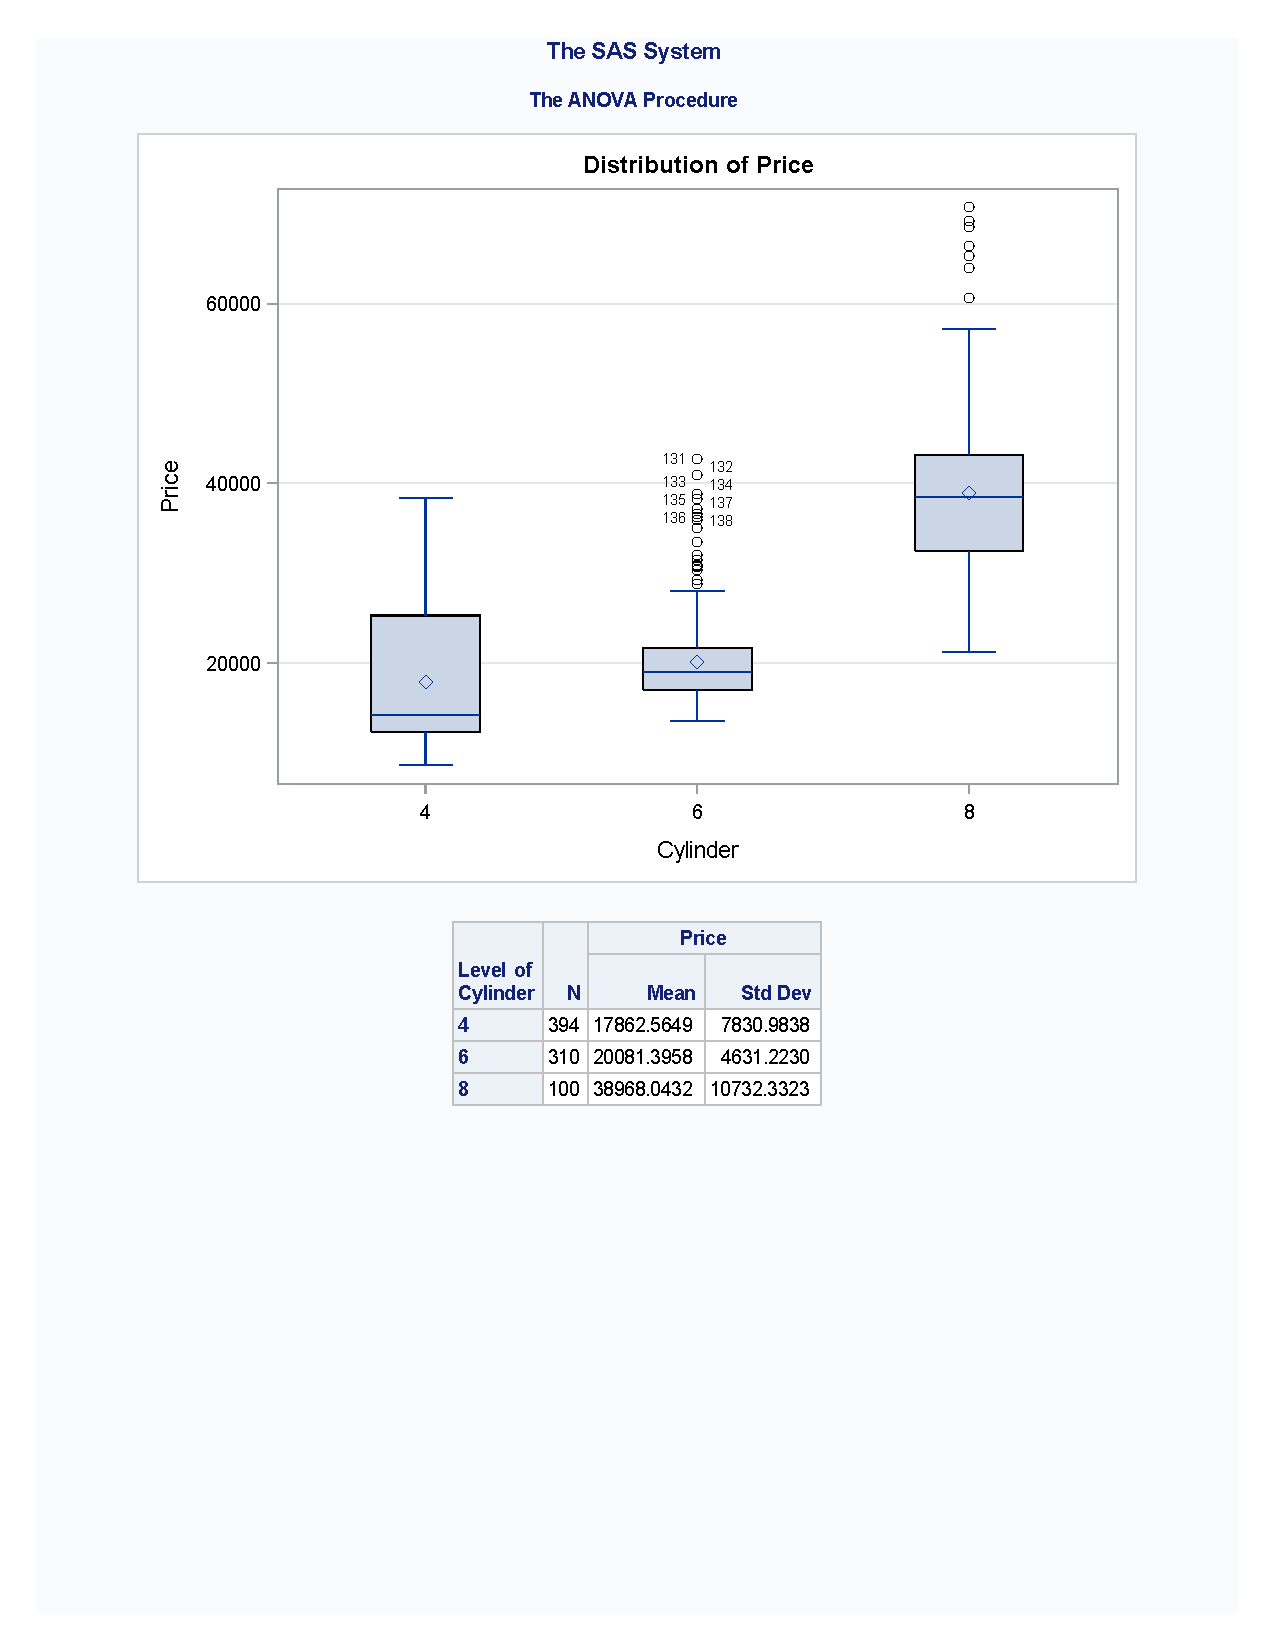
\includegraphics[trim=7cm 9cm 7cm 15cm,clip,width=1.0\textwidth]{L13_anova3.pdf}
\emp
\end{frame}



\begin{frame}
\frametitle{Conditions for one-way ANOVA}
\begin{enumerate}
    \item
    observations are independent (in each of the $g$ groups)
    \item
    normal underlying population distribution OR $n \geq 30$ in each group
    \item
    each group has (about) the same variability (equal variance)
\end{enumerate}
\vskip10pt
\oyo How would you check these conditions?
\end{frame}


\begin{frame}
\ft{\ttt{MEANS} options}
	\bi
	\item Many multiple comparison methods available: \ttt{TUKEY}, \ttt{SCHEFFE}, \ttt{DUNCAN}, \ttt{BON} (for Bonferroni).
	\item \fbox{\ttt{ALPHA=}} controls overall error rate
	\item To test the assumption of equal variance, use the \fbox{\ttt{HOVTEST}} option (\ttb{\underline{H}}omogeneity \ttb{\underline{O}}f \ttb{\underline{V}}ariance test). For this test, the null hypothesis is $H_0$: Variances are equal. Smaller p-values lend stronger evidence against this statement.
		%\item \fbox{\ttt{LINES}} -- When possible, SAS will align the various treatments in a column and `connect' all treatments that are not significantly different.
	\ei
\end{frame}

\begin{frame}[fragile]
\frametitle{PROC ANOVA Example, continued}
\bmp{0.55\textwidth}
\footnotesize
\begin{code}{.0}
PROC ANOVA DATA = flash.cars ;
   CLASS cylinder ;
   MODEL price = cylinder ;
   MEANS cylinder
   / TUKEY HOVTEST ;
QUIT ;
\end{code}
\vspace{2ex}
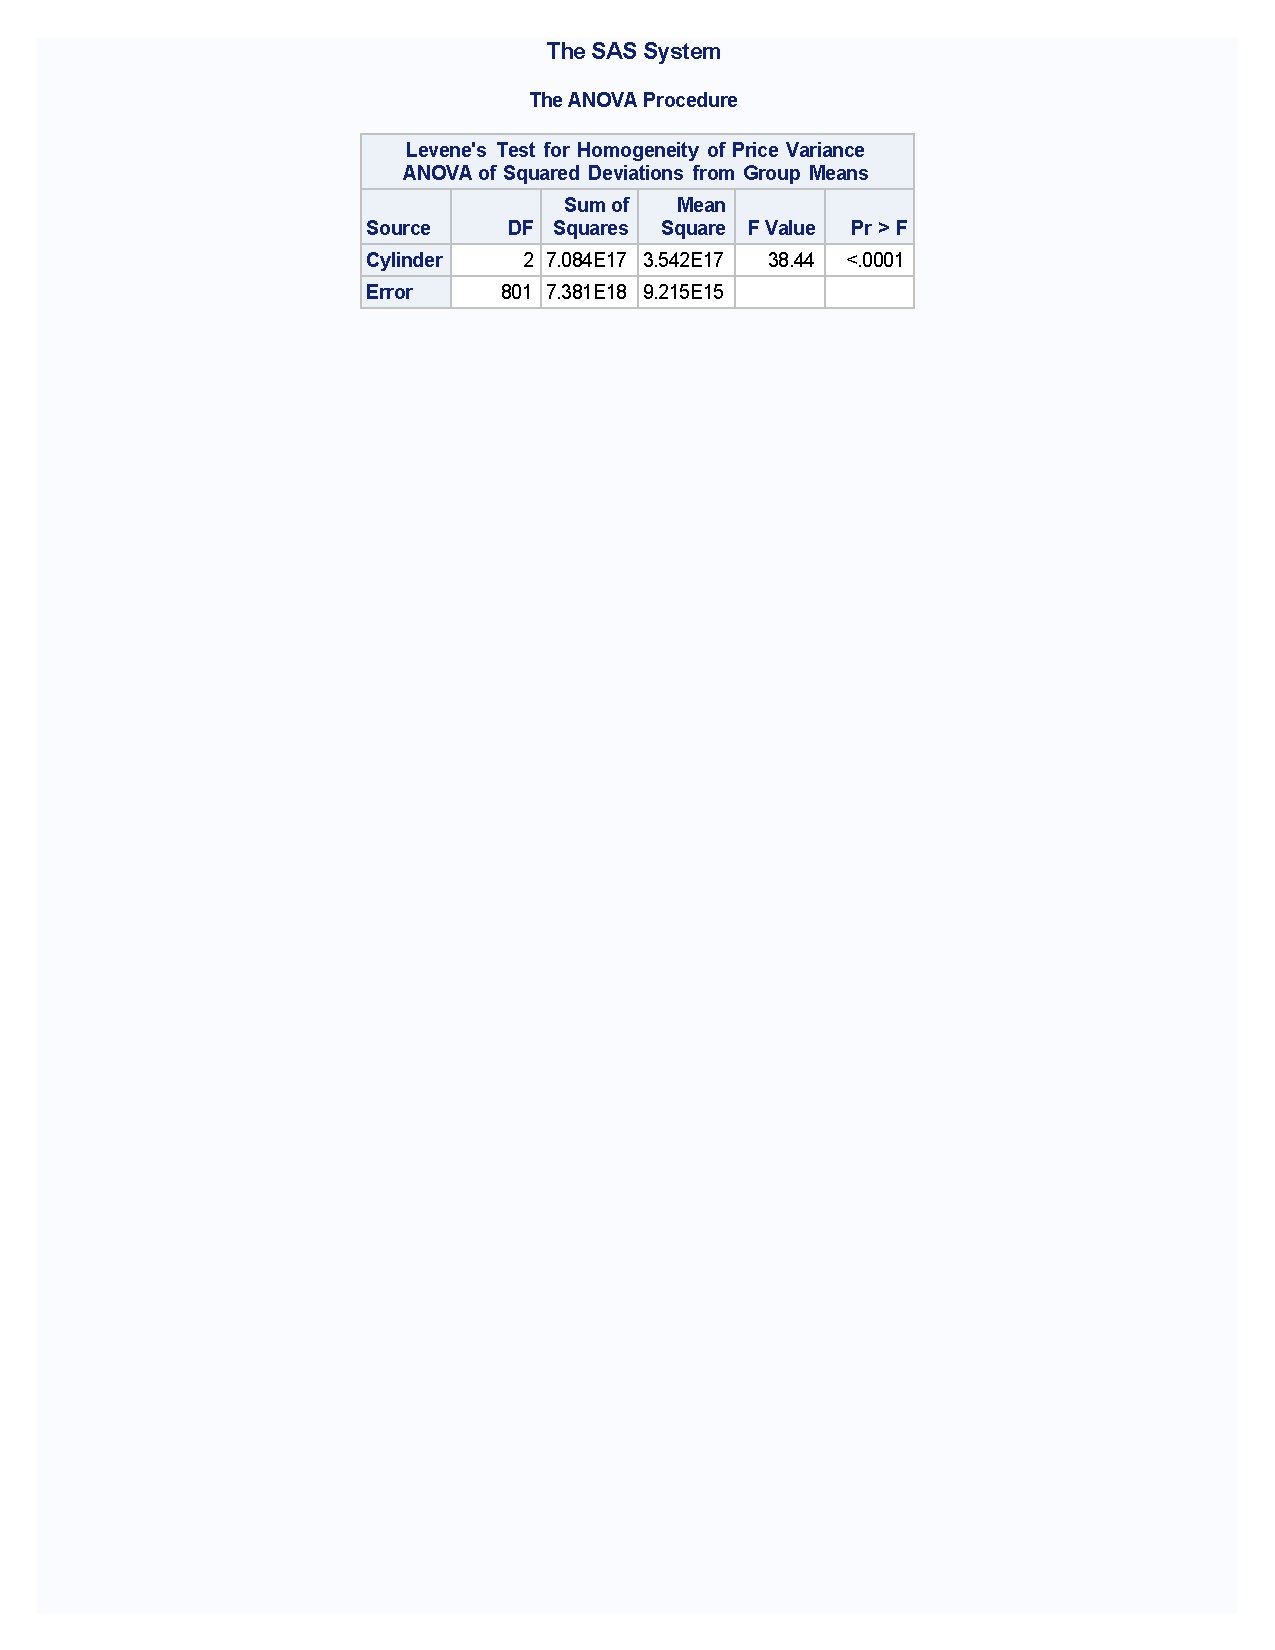
\includegraphics[trim=5cm 22cm 5cm 2cm,clip,width=1.0\textwidth]{L13_anova_mc3.pdf}
\emp
\bmp{0.05\textwidth} \hspace{1in} \emp
\bmp{0.45\textwidth}
\oyo Is the equality of variance condition satisfied?  For which cylinder comparisons do we have evidence of a difference in population mean price?\\
\vskip5pt
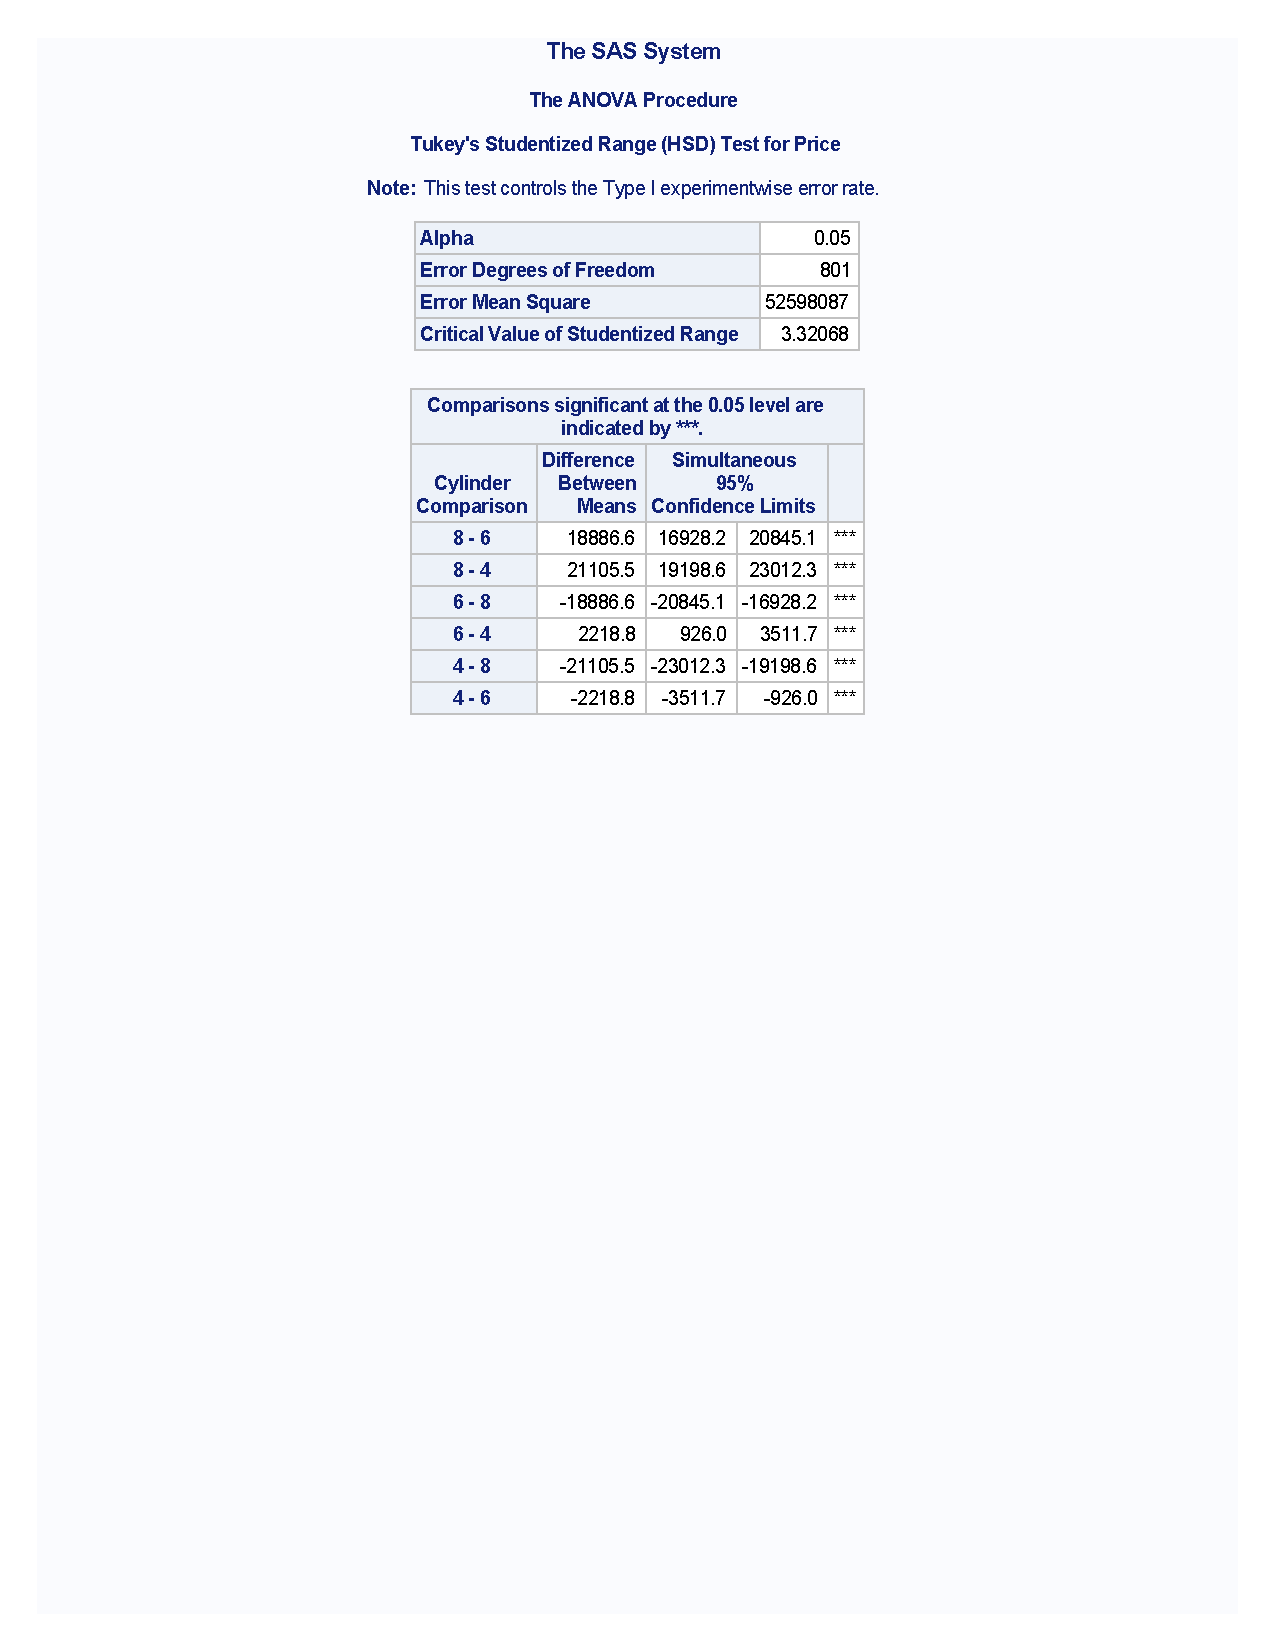
\includegraphics[trim=6cm 15cm 6cm 6.0cm,clip,width=1.0\textwidth]{L13_anova_mc5a.pdf}
\emp

\end{frame}

\begin{frame}[fragile]
\ft{The same analysis, but with PROC GLM}
\bmp{0.55\textwidth}
\begin{code}{.0}
PROC GLM DATA = flash.cars ;
   CLASS cylinder ;
   MODEL price = cylinder ;
QUIT ;
\end{code}
\emp
\bmp{0.05\textwidth} \hspace{1in} \emp
\bmp{0.45\textwidth}
\begin{itemize}
\item same base output as \texttt{PROC ANOVA}
\item requires much more work to get multiple comparisons
\end{itemize}
\emp
\end{frame}

\begin{frame}
\frametitle{Warning}
\bi
\item  the ANOVA procedure is designed to handle \emph{balanced data} (groups with equal sample sizes)
\bi
\item for one-way ANOVA, \ttt{PROC ANOVA} still works ok even for unbalanced data
\ei
\item if you have unbalanced data and you want to do something more complex than one-way ANOVA, use \ttt{PROC GLM}
\ei
\vskip10pt
\begin{clicker}{Was \ttt{PROC ANOVA} valid for analyzing the relationship between \ttt{price} and \ttt{cylinder}?}
\begin{enumerate}
    \item Yes
    \item No
\end{enumerate}
\end{clicker}
\end{frame}


%===========================================================================================================================
\section[Regression]{Regression}
%===========================================================================================================================
\subsection{}
\begin{frame}
\tableofcontents[currentsection, hideallsubsections]
\end{frame}

\begin{frame}
\ft{Review}
\begin{clicker}{Which figure would you produce to examine the relationship between \texttt{price} and \texttt{mileage}?}
\begin{enumerate}
\item histogram
\item single boxplot
\item side by side boxplot
\item scatter plot
\end{enumerate}
\end{clicker}
\end{frame}

\begin{frame}[fragile]
\frametitle{Relationship between price and mileage}
Both \ttt{PROC REG} and \ttt{PROC GLM} can be used for simple linear regression with a quantitative independent variable.
\vskip5pt
\bmp{0.5\textwidth}
\footnotesize
\begin{code}{.0}
PROC REG DATA = flash.cars ;
   MODEL price = mileage ;
QUIT ;

PROC GLM DATA = flash.cars ;
  MODEL price = mileage ;
QUIT ;
\end{code}
\emp
\bmp{0.05\textwidth} \hspace{1in} \emp
\bmp{0.5\textwidth}
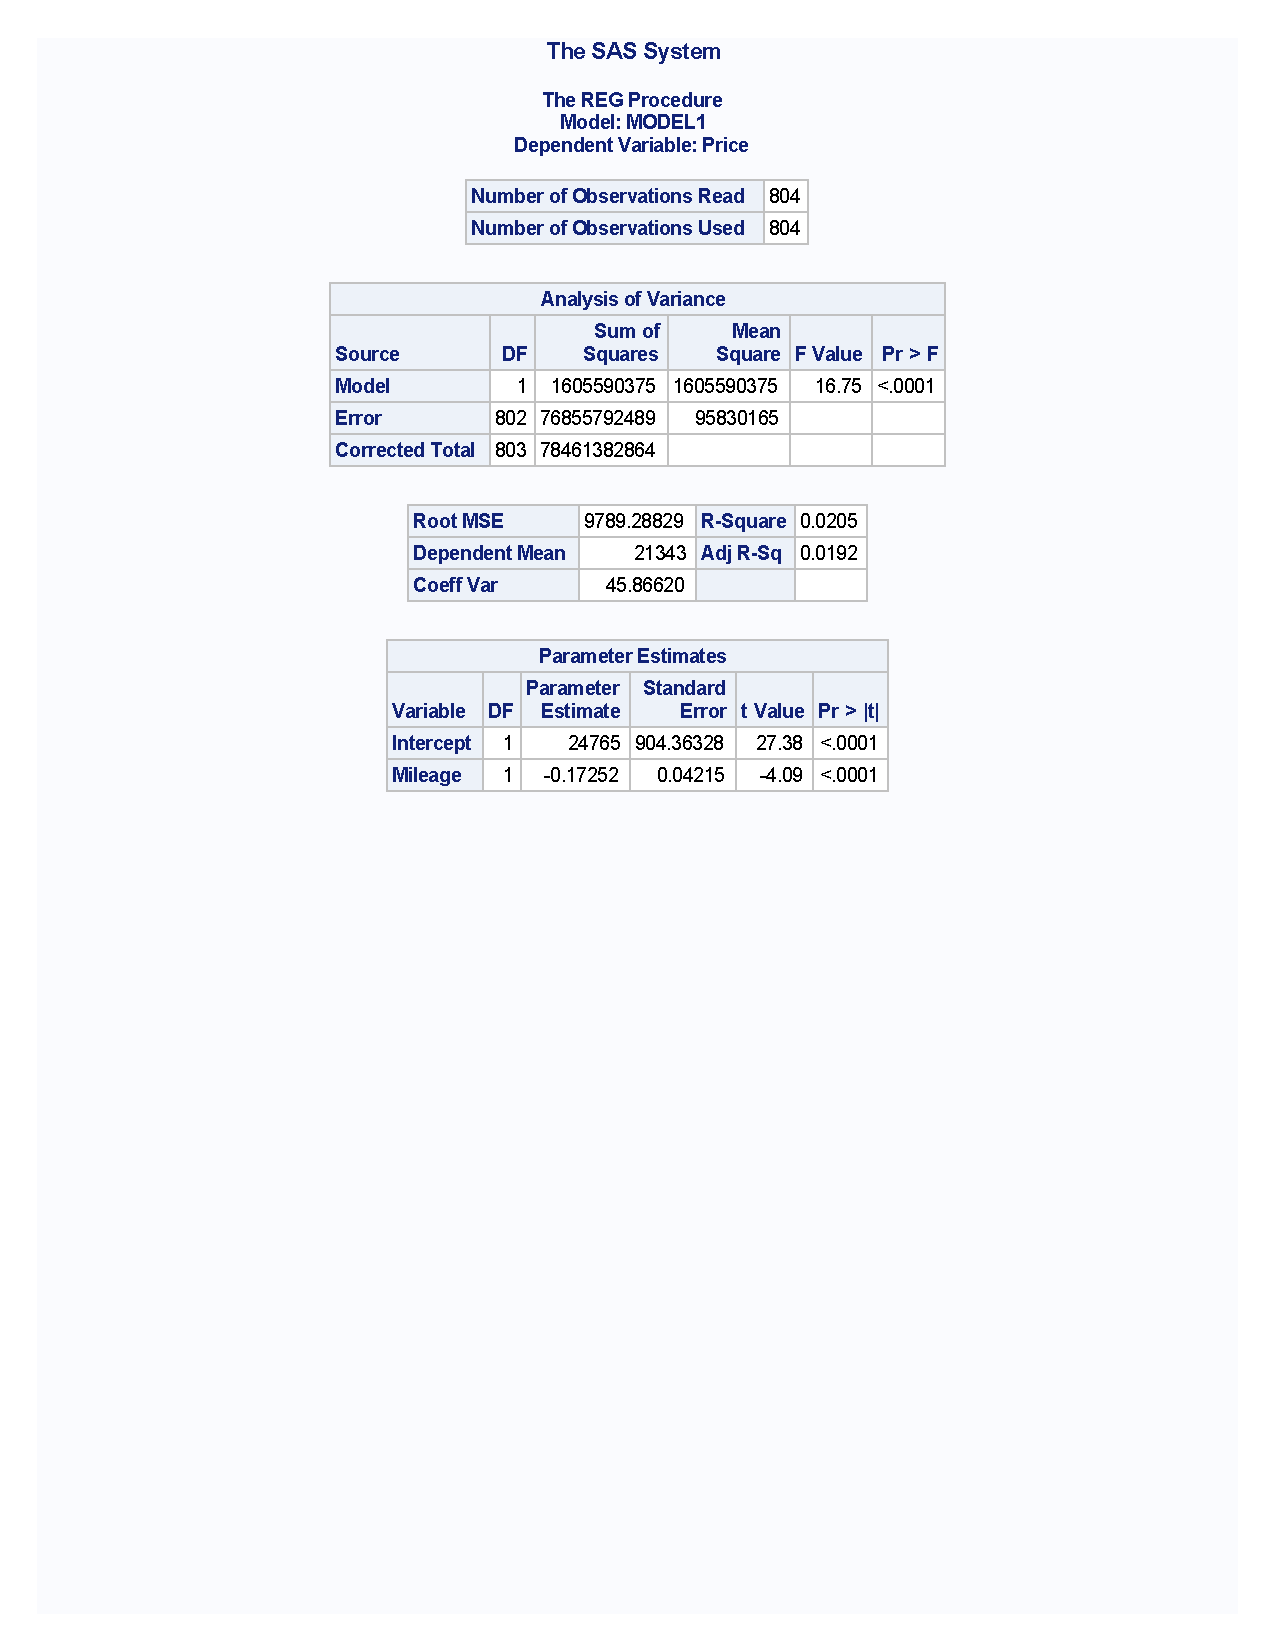
\includegraphics[trim=5cm 13cm 5cm 1.2cm,clip,width=1.0\textwidth]{L13_reg.pdf}
\emp
\end{frame}

\begin{frame}[fragile]
\frametitle{Other features of PROC REG - multiple model statements}
\bmp{1.0\textwidth}
\footnotesize
\begin{code}{.0}
PROC REG DATA = flash.cars ;
   MODEL price = mileage ;
   MODEL price = liter ;
QUIT ;
\end{code}
\emp
\end{frame}

\begin{frame}[fragile]
\frametitle{Other features of PROC REG - create data set with residuals and other diagnostic measures}
\bmp{1.05\textwidth}
\footnotesize
\begin{code}{.0}
PROC REG DATA = flash.cars ;
   MODEL price = mileage ;
   OUTPUT OUT = reg_results PREDICTED = yhat RESIDUAL = resid ;
QUIT ;

PROC PRINT DATA = reg_results (obs = 5) ;
    VAR price mileage yhat resid ;
RUN ;
\end{code}
\vskip5pt
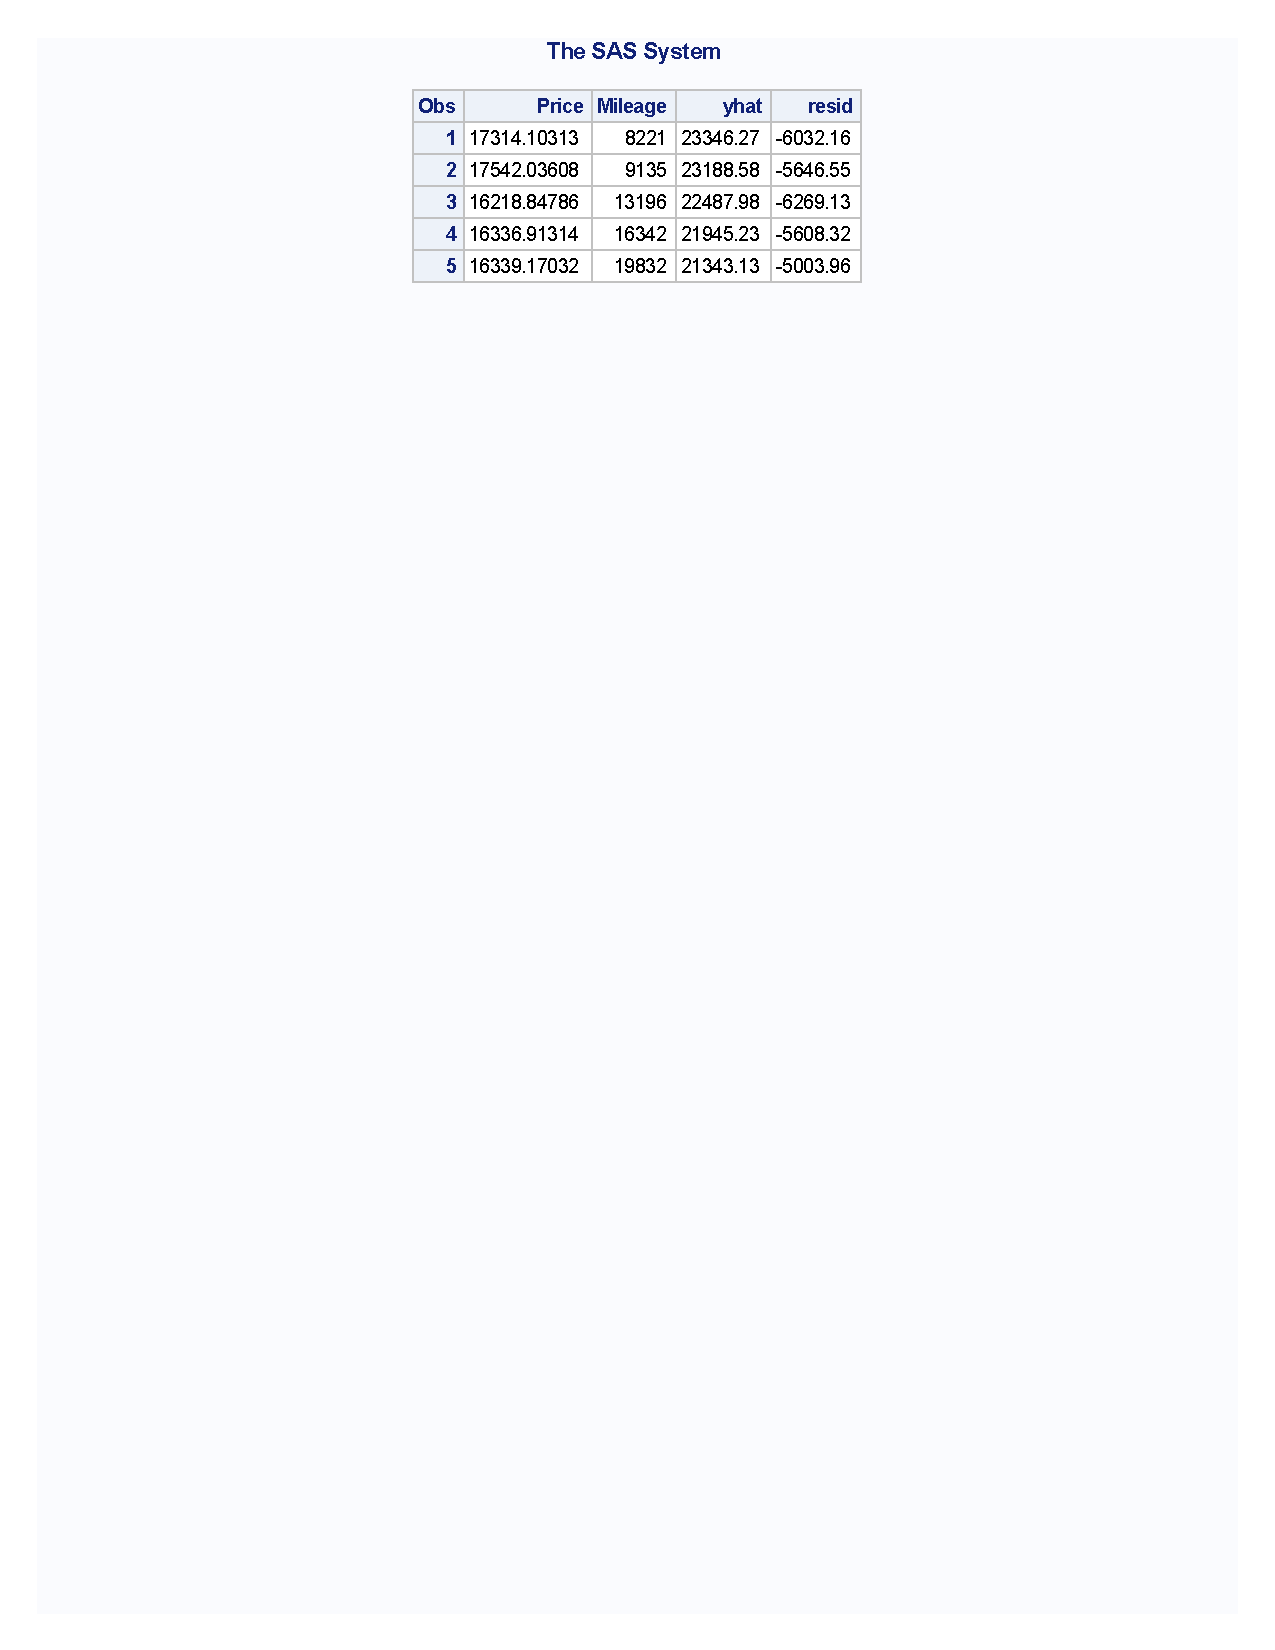
\includegraphics[trim=6cm 18cm 7cm 1.2cm,clip, width=0.40\textwidth]{L13_resid.pdf}
\emp
\end{frame}

\begin{frame}
\ft{PROC REG confidence limits}
\fbox{\ttt{MODEL \emph{quantvar} = \emph{independent var(s)} / \textcolor{OrangeRed}{\emph{options}};}}
\vskip10pt
Confidence interval options include:
\bi
\item \ttt{CLB} - confidence limits for parameters
\item \ttt{CLI} - confidence limits for an individual predicted value
\item \ttt{CLM} - confidence limits for an average/expected value of dependent variable
\ei
\end{frame}


\begin{frame}[fragile]
\ft{\small{Relationship between price and mileage, adjusting for sound}}
This model can be executed in either \ttt{PROC REG} or \ttt{PROC GLM} because \ttt{sound} is coded as 0/1 (an indicator variable).
\vskip10pt
\bmp{0.55\textwidth}
\footnotesize
\begin{code}{.0}
PROC REG DATA = flash.cars ;
   MODEL price = mileage sound ;
QUIT ;

PROC GLM DATA = flash.cars ;
  MODEL price = mileage sound ;
QUIT ;
\end{code}
\emp
\bmp{0.05\textwidth} \hspace{1in} \emp
\bmp{0.45\textwidth}
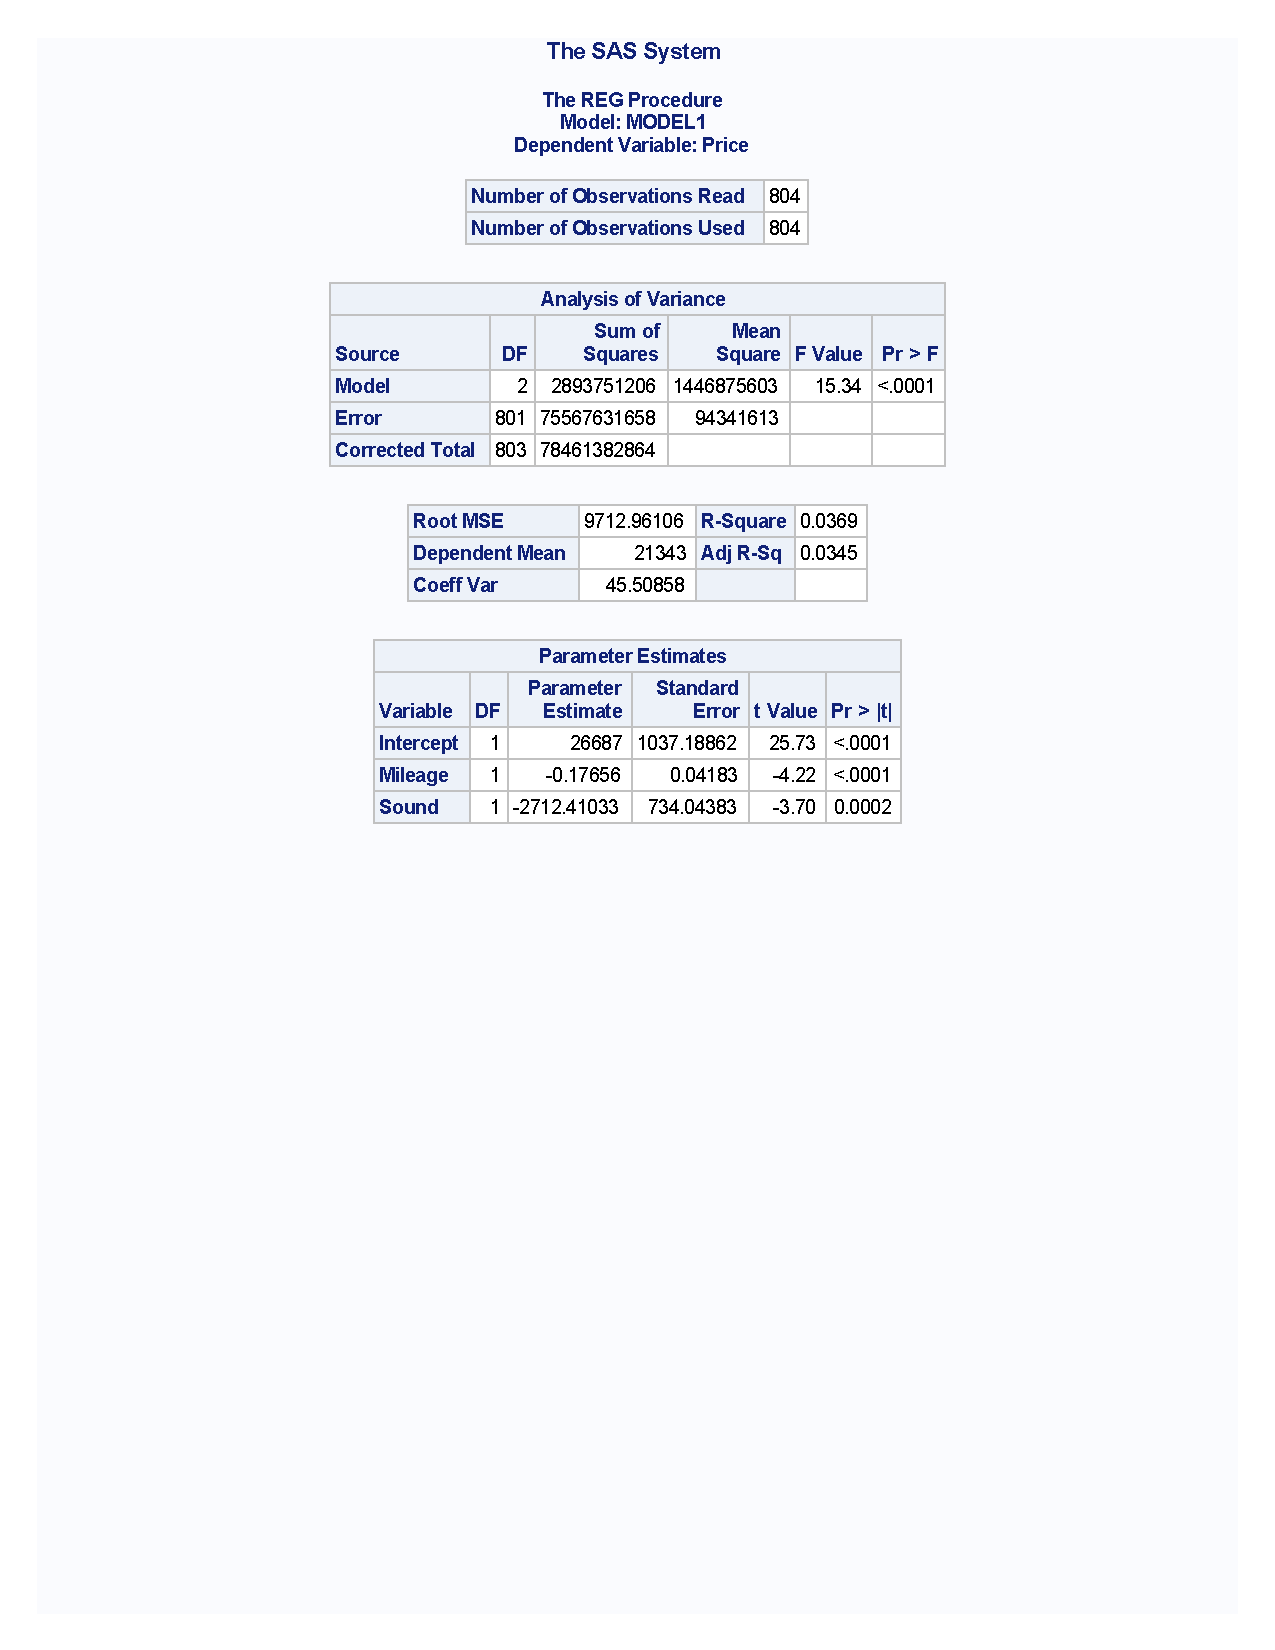
\includegraphics[trim=5cm 13cm 5cm 1.2cm,clip,width=1.0\textwidth]{L13_sound.pdf}
\emp
\end{frame}

\begin{frame}[fragile]
\frametitle{Relationship between price and mileage, adjusting for cruise}
This model can only be executed in \ttt{PROC GLM} because \ttt{cruise} is coded as Y/N.
\vskip5pt
\bmp{1.0\textwidth}
\footnotesize
\begin{code}{.0}
PROC GLM DATA = flash.cars ;
  \textcolor{OrangeRed}{CLASS cruise ;}
  MODEL price = mileage cruise / \textcolor{OrangeRed}{SOLUTION} ;
QUIT ;
\end{code}
\emp
\vskip5pt
\bi
\item Use the \ttt{CLASS} statement for the categorical variable
\item Use \ttt{SOLUTION} option to obtain parameter estimates
\item You could do this with \ttt{PROC REG} if you coded \ttt{cruise} as 0/1 in the data set
\ei
\end{frame}

\begin{frame}[fragile]
\frametitle{Exploring a quadratic relationship with mileage}
This model can be easily executed in \ttt{PROC GLM}.
\vskip5pt
\bmp{1.0\textwidth}
\footnotesize
\begin{code}{.0}
PROC GLM DATA = flash.cars ;
  MODEL price = mileage \textcolor{OrangeRed}{mileage*mileage} ;
QUIT ;
\end{code}
\emp
\vskip5pt
\bi
\item You could do this with \ttt{PROC REG} if you coded \ttt{mileage\_squared} in the data set
\item The same idea applies to interaction terms (\ttt{PROC GLM} can handle them in the model statement, \ttt{PROC REG} needs the variables to be coded in the data set)
\ei
\end{frame}

\begin{frame}[fragile]
\ft{PROC REG model selection}
Another \emph{option} for the \ttt{MODEL} statement in \ttt{PROC REG} allows you to do automated model selection.  There are 9 model selection methods available.
\vskip5pt
\bmp{1.0\textwidth}
\footnotesize
\begin{code}{.0}
PROC REG DATA = flash.cars ;
  MODEL price = mileage liter sound leather /
     \textcolor{OrangeRed}{SELECTION = RSQUARE} ;
QUIT ;
\end{code}
\emp
\vskip5pt
This example uses the R-squared method to examine all possible models based on the 4 independent variables.
\end{frame}

\begin{frame}
\ft{Conditions for regression}
\begin{enumerate}
\item observations are independent
\item linear relationship between $x$ and $y$
\item normally distributed errors about the regression line
\item constant variability in $y$ about the regression line (constant variance)
\item[]
\end{enumerate}
\oyo How would you check these conditions?
\end{frame}

\end{document} 